\section{Diseño de la interfaz gráfica de usuario}
\addcontentsline{toc}{section}{Diseño de la interfaz gráfica de usuario}
\textbf{Análisis de aplicaciones similares}: No es posible mejorar un producto sin analizarlo y criticarlo. Por ende, es necesario comparar el diseño del prototipo del interfaz gráfica de usuario para así mejorarlo en términos de usabilidad y comodidad.

Las aplicaciones que se van a utilizar como objectos de comparación son las mismas que se utilizaron en los antecedentes, \textit{FAT - Frame Data!} y \textit{Smash Ultimate Calculator}.

Como se puede apreciar en la figuras \ref{fig: char sel}, \ref{fig: game select}, \ref{fig: compare options} y \ref{fig: comparison}, \textit{FAT - FRAME DATA!} parece utilizar diseño material \cite{noauthor_designing_nodate}. Mas aún, en la figura \ref{fig: char sel}, se utilizan las siluetas de los personajes con el color predominante del personaje como color de fondo. Esto ayuda reducir la carga de memoria de los usuarios mientras que no sacrifica mucho en términos de usabilidad. Es una buena decisión de diseño y es algo que falta en la interfaz gráfica de usuario de SkyboundDB 2.0. Al utilizar principios del diseño material, \textit{FAT - Frame Data!} es inmediatamente familiar a usuarios de aplicaciones de \textit{Google} y \textit{Android}. El uso de diseño material fue una buena decisión de diseño ya que facilita la adaptación de los usuarios a una aplicación nueva porque comparte principios y estándares de diseño.

\begin{figure}
    \centering
    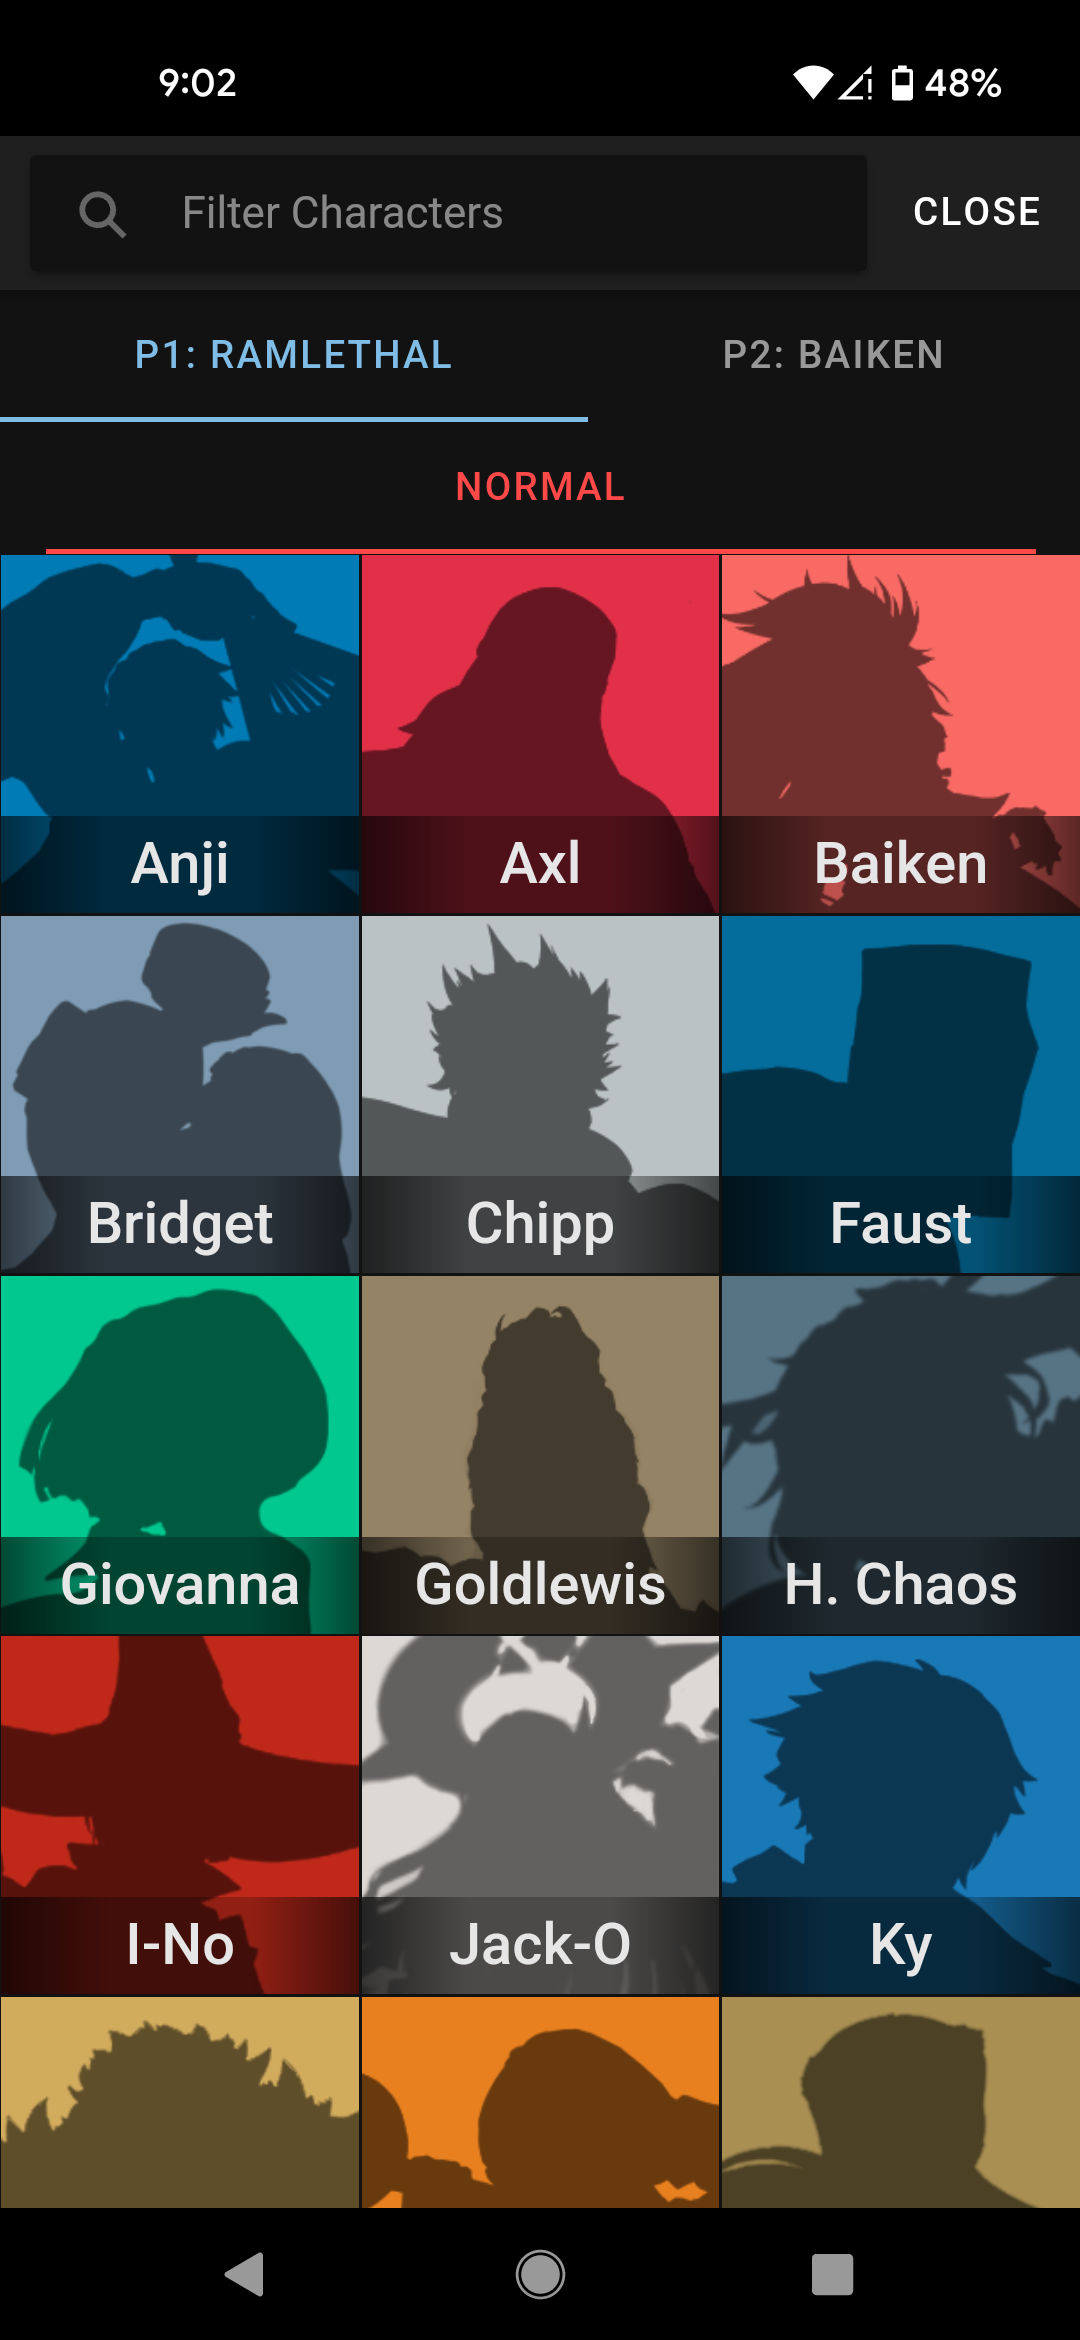
\includegraphics[height=0.4\textheight]{figures/char_sel.png}
    \caption{Selección de personaje en \textit{FAT - FRAME DATA!}}
    \label{fig: char sel}
\end{figure}

\begin{figure}
    \centering
    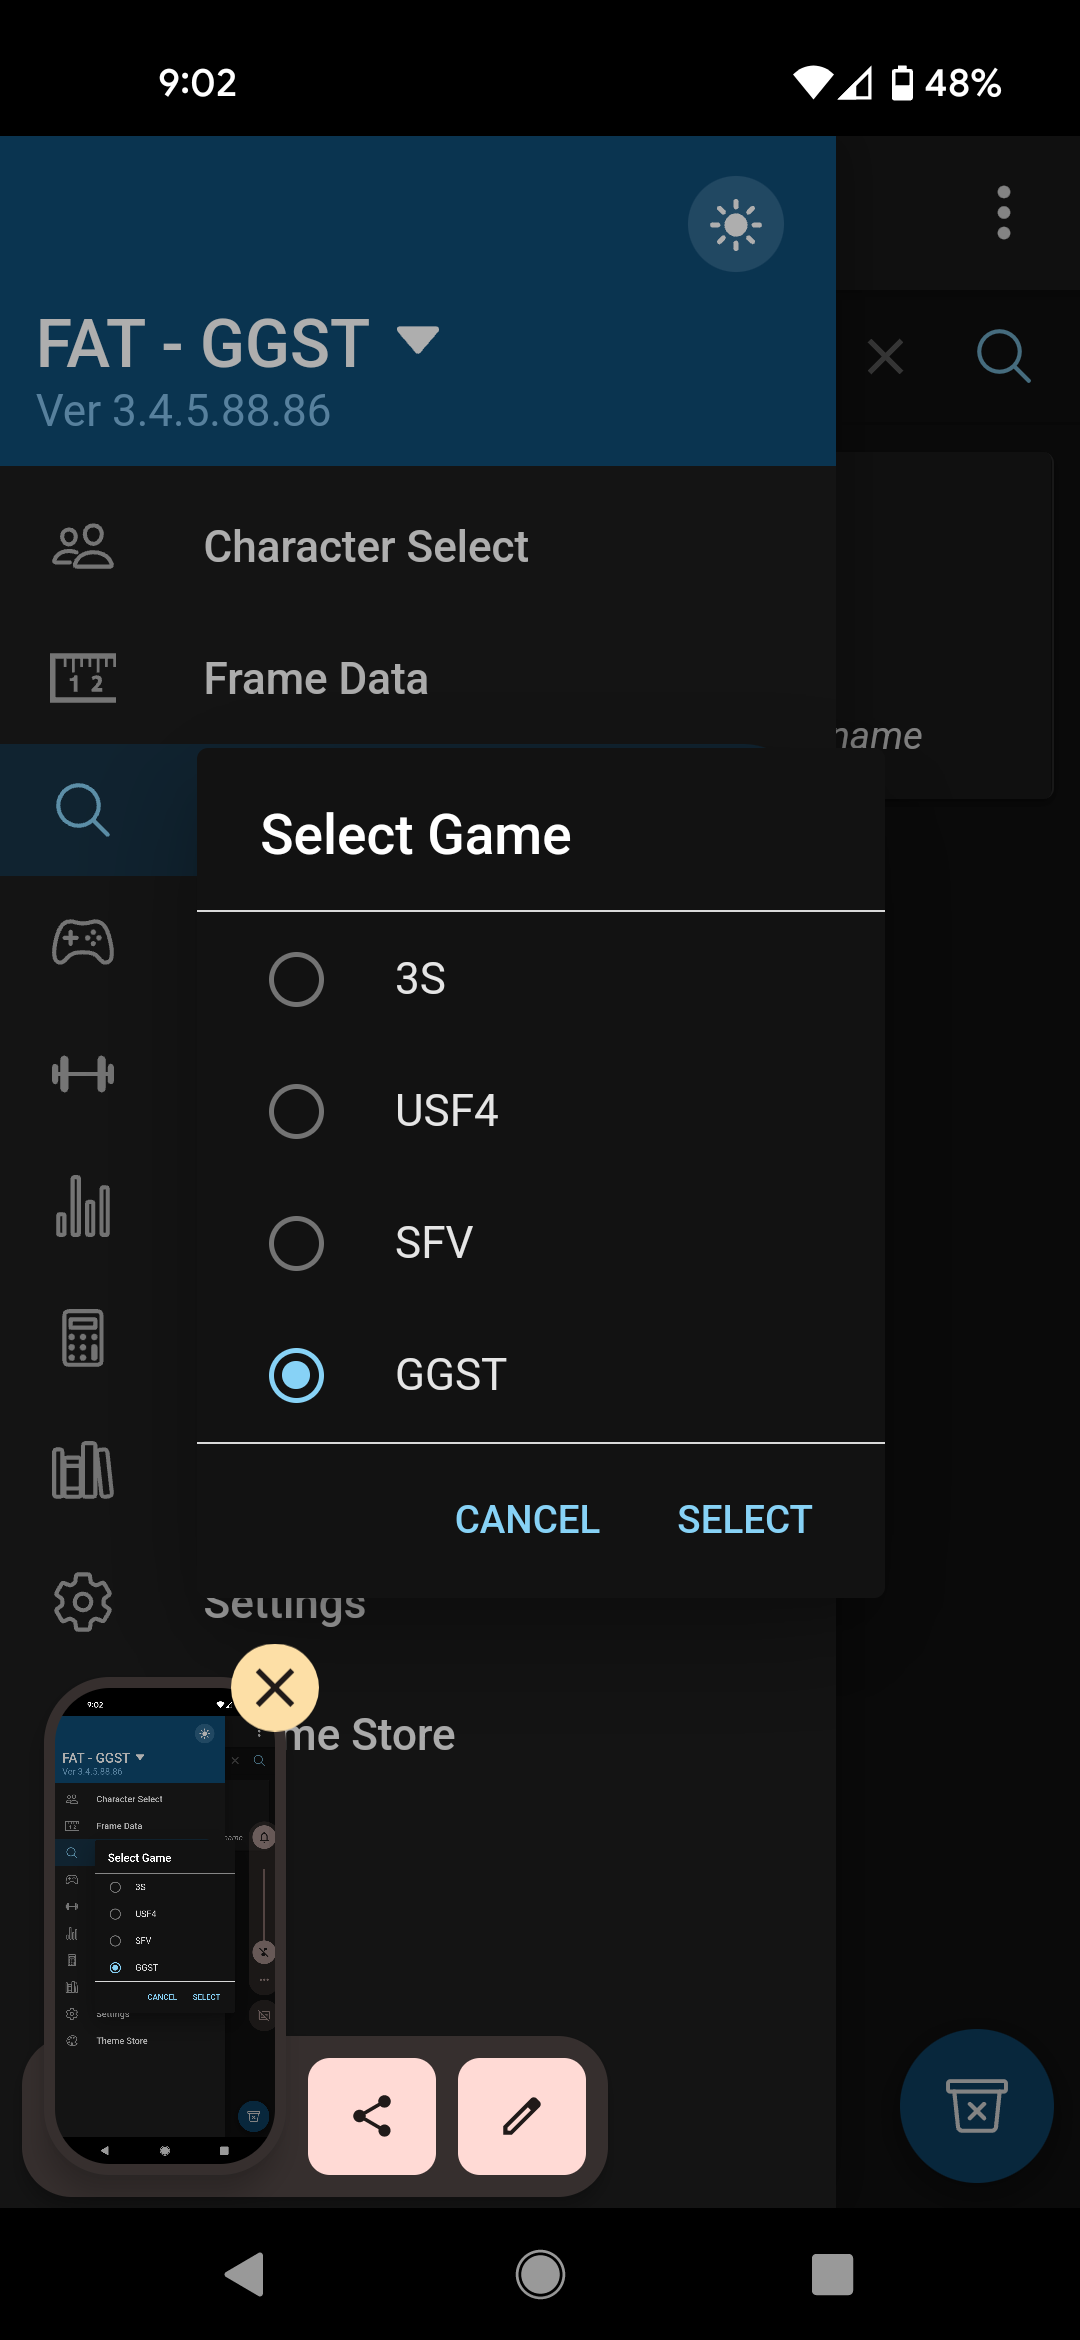
\includegraphics[height=0.4\textheight]{figures/game_options.png}
    \caption{Selección de juego en \textit{FAT - FRAME DATA!}}
    \label{fig: game select}
\end{figure}

\begin{figure}
    \centering
    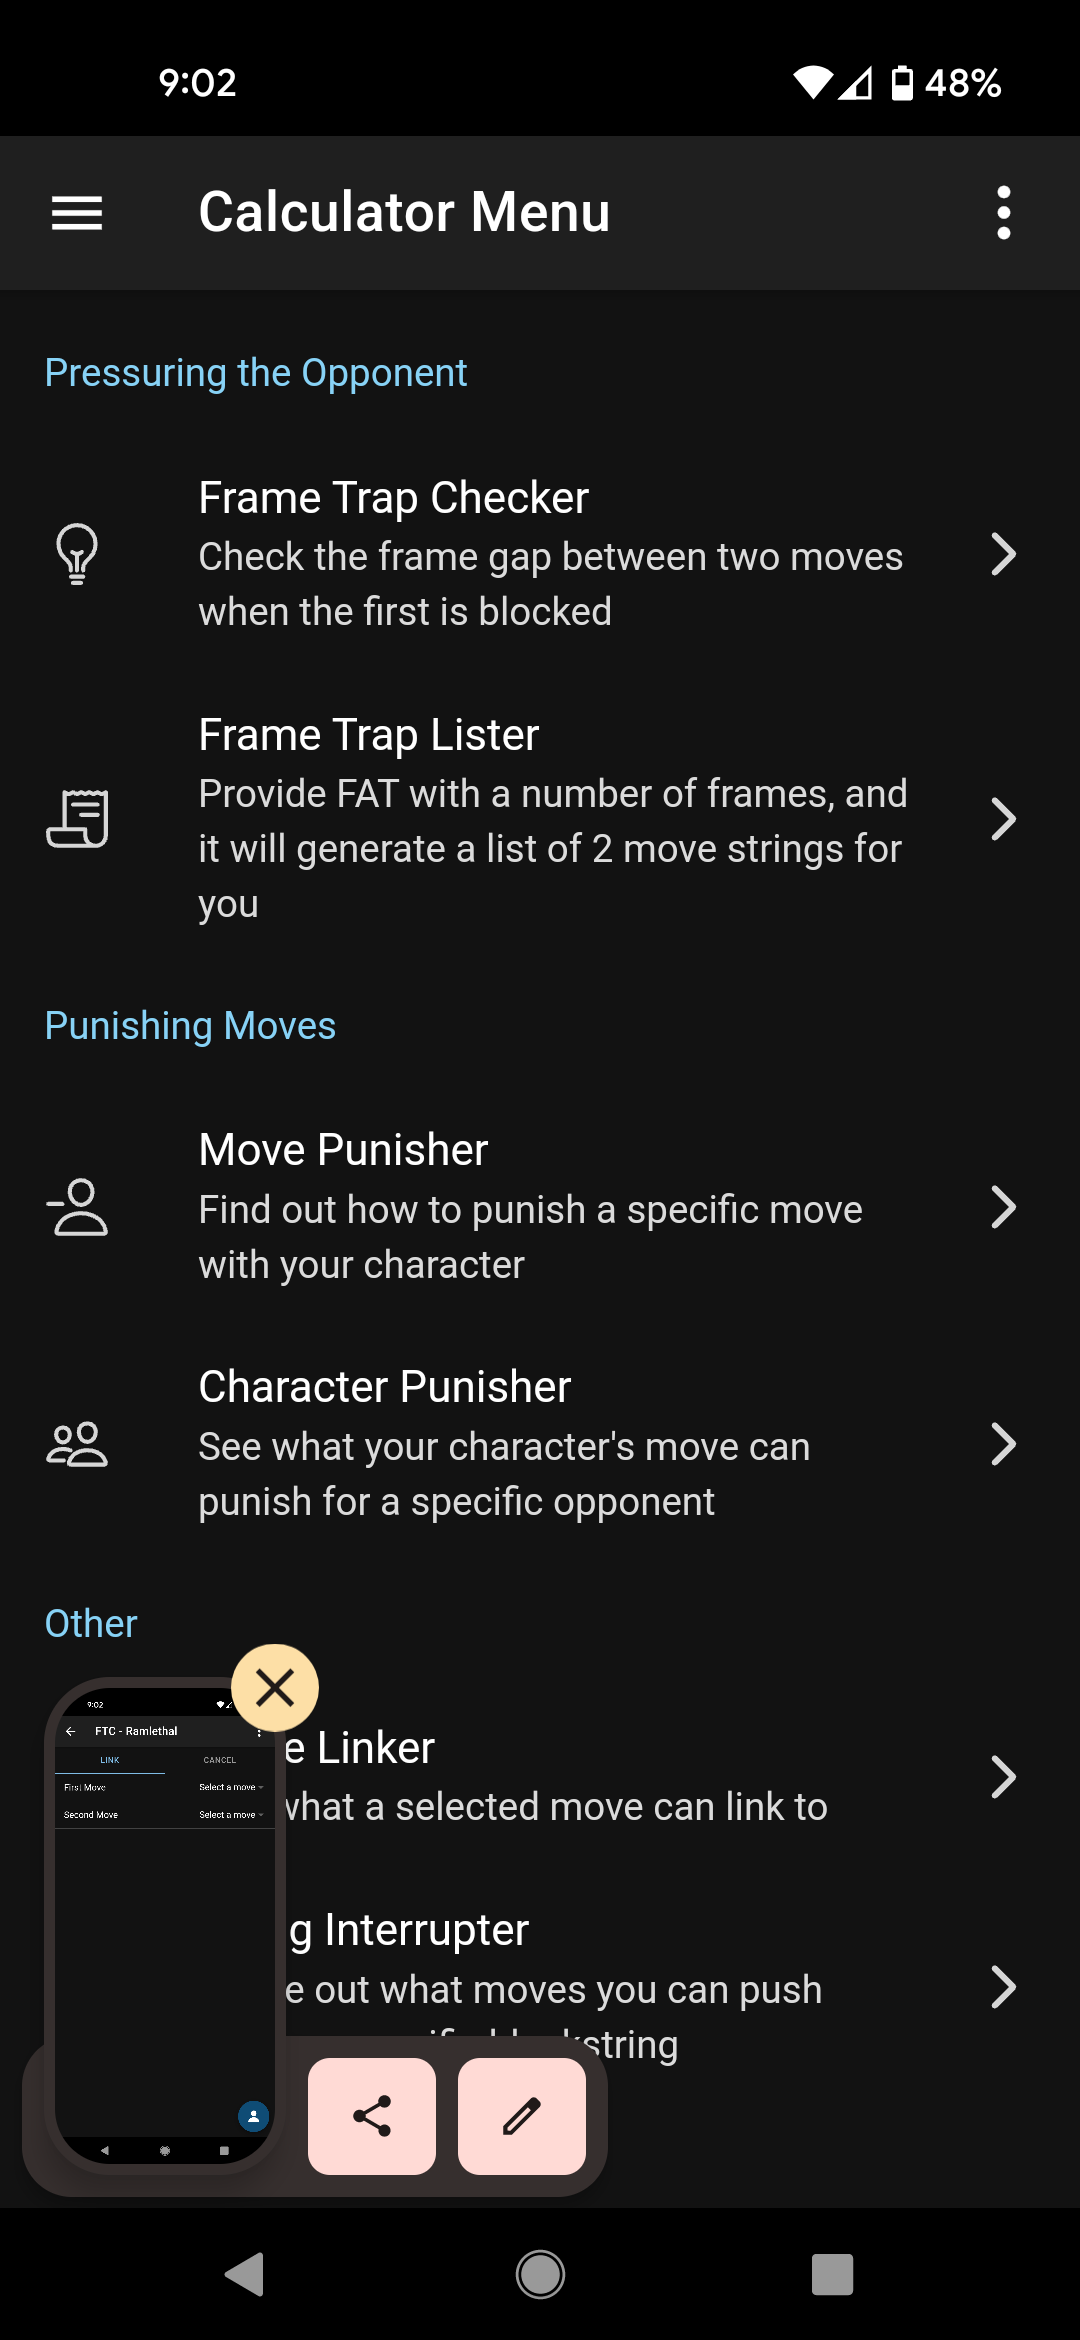
\includegraphics[height=0.4\textheight]{figures/compare_options.png}
    \caption{Opciones de comparación en \textit{FAT - FRAME DATA!}}
    \label{fig: compare options}
\end{figure}

\begin{figure}
    \centering
    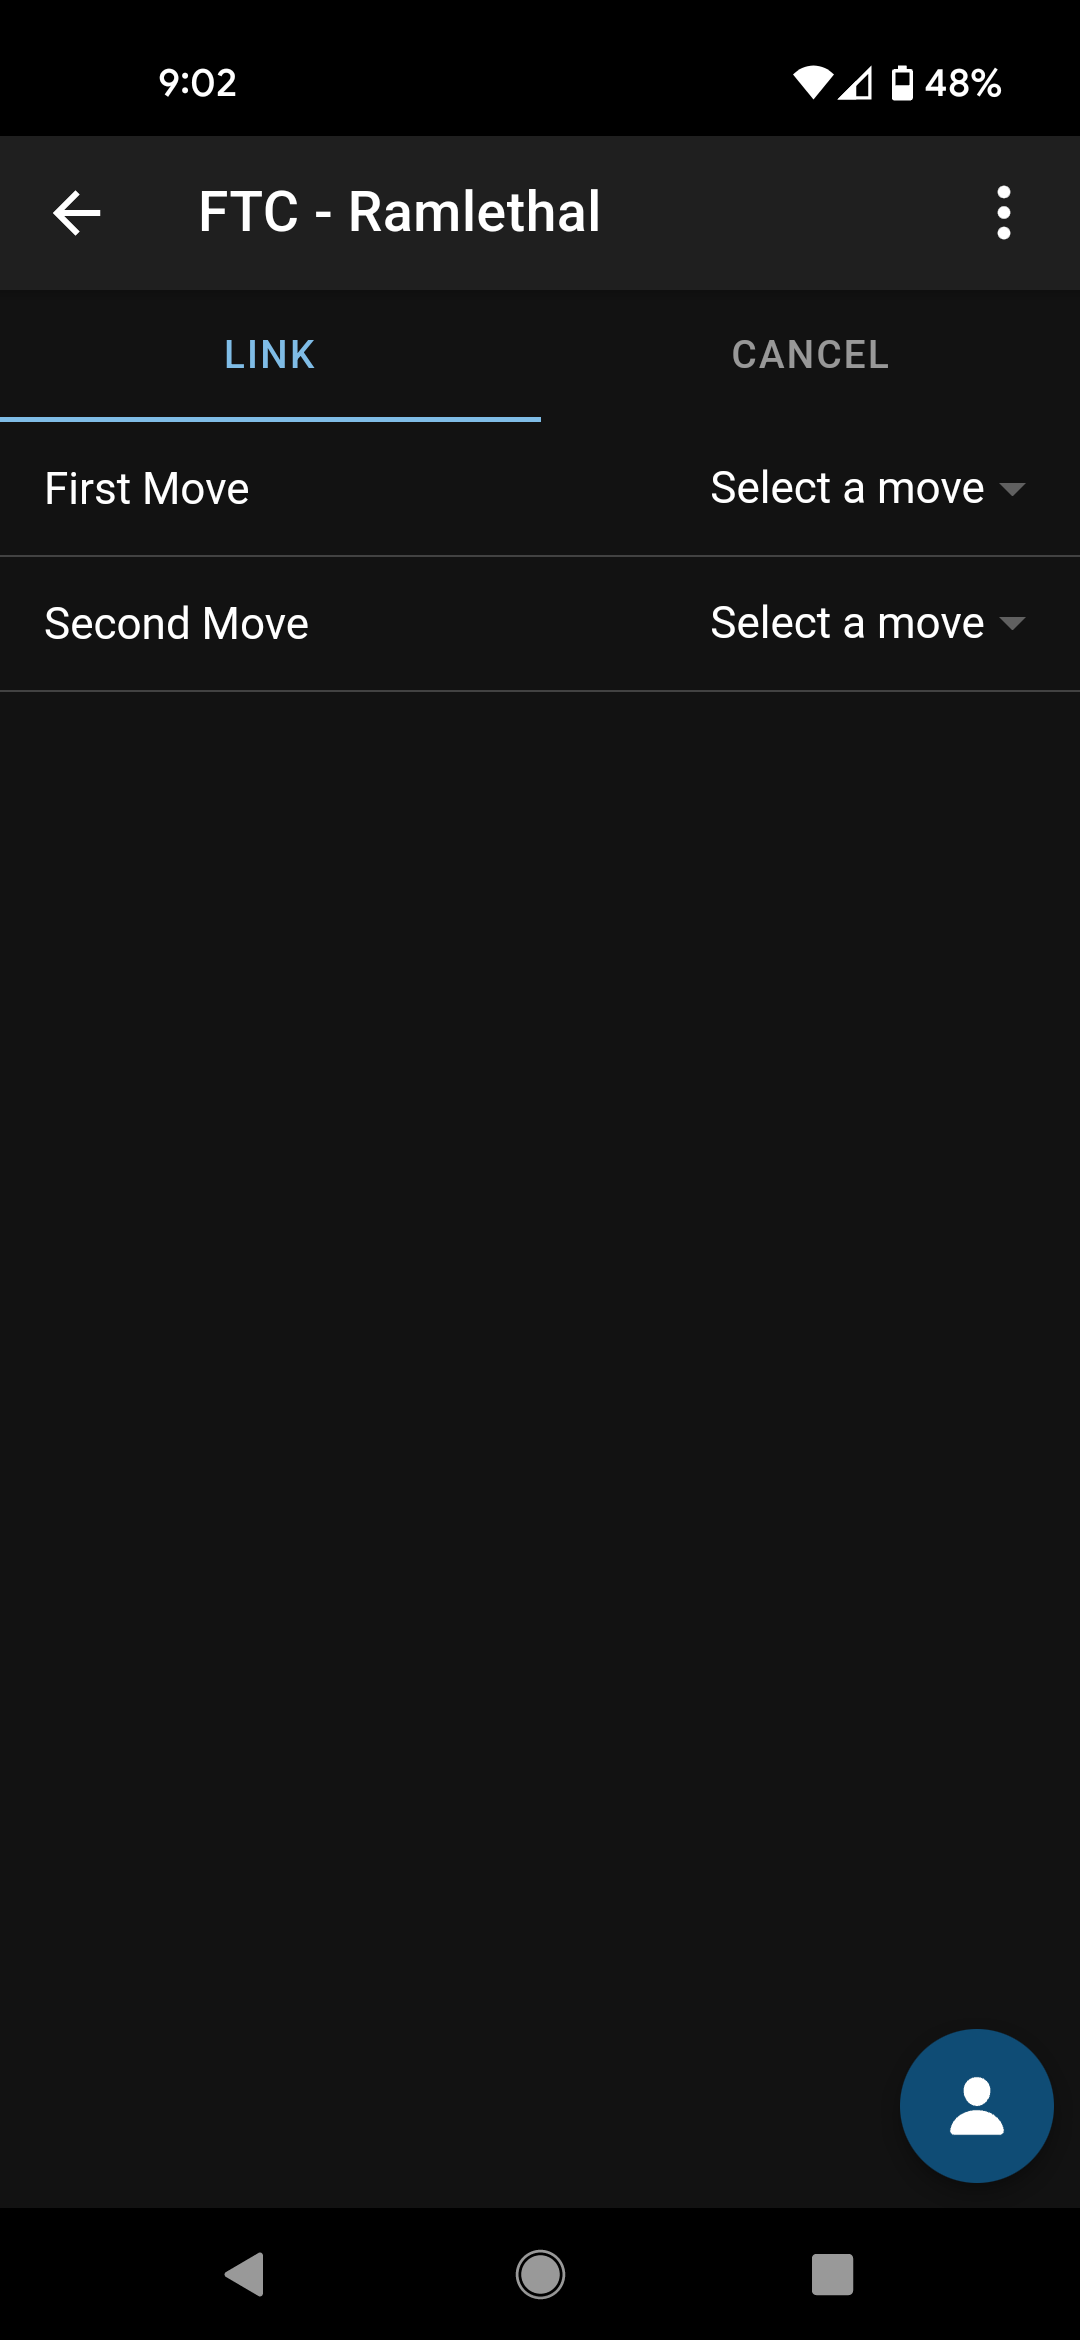
\includegraphics[height=0.4\textheight]{figures/comparison.png}
    \caption{Comparación entre movidas en \textit{FAT - FRAME DATA!}}
    \label{fig: comparison}
\end{figure}

\newpage

\textit{Smash Ultimate Calculator} no parece utilizar un estándar de diseño al igual que SkyboundDB 2.0. Esto crea confusión al utilizar la aplicación por primera vez. Como se puede ver en las figuras \ref{fig: SUC main menu} y \ref{fig: SUC additional options}, a pesar que las áreas que contienen información están agrupadas lógicamente, hay demasiados elementos y opciones que se presentan al usuario. Esto incurre una gran carga de memoria e intimida al usuario novato. También es difícil ver que cambios ocurren al oprimir opciones. A pesar de estas decisiones de diseño problemáticas, la paleta de colores es pasable, sino un poco deprimente y sin vida.

\begin{figure}[ht!]
    \centering
    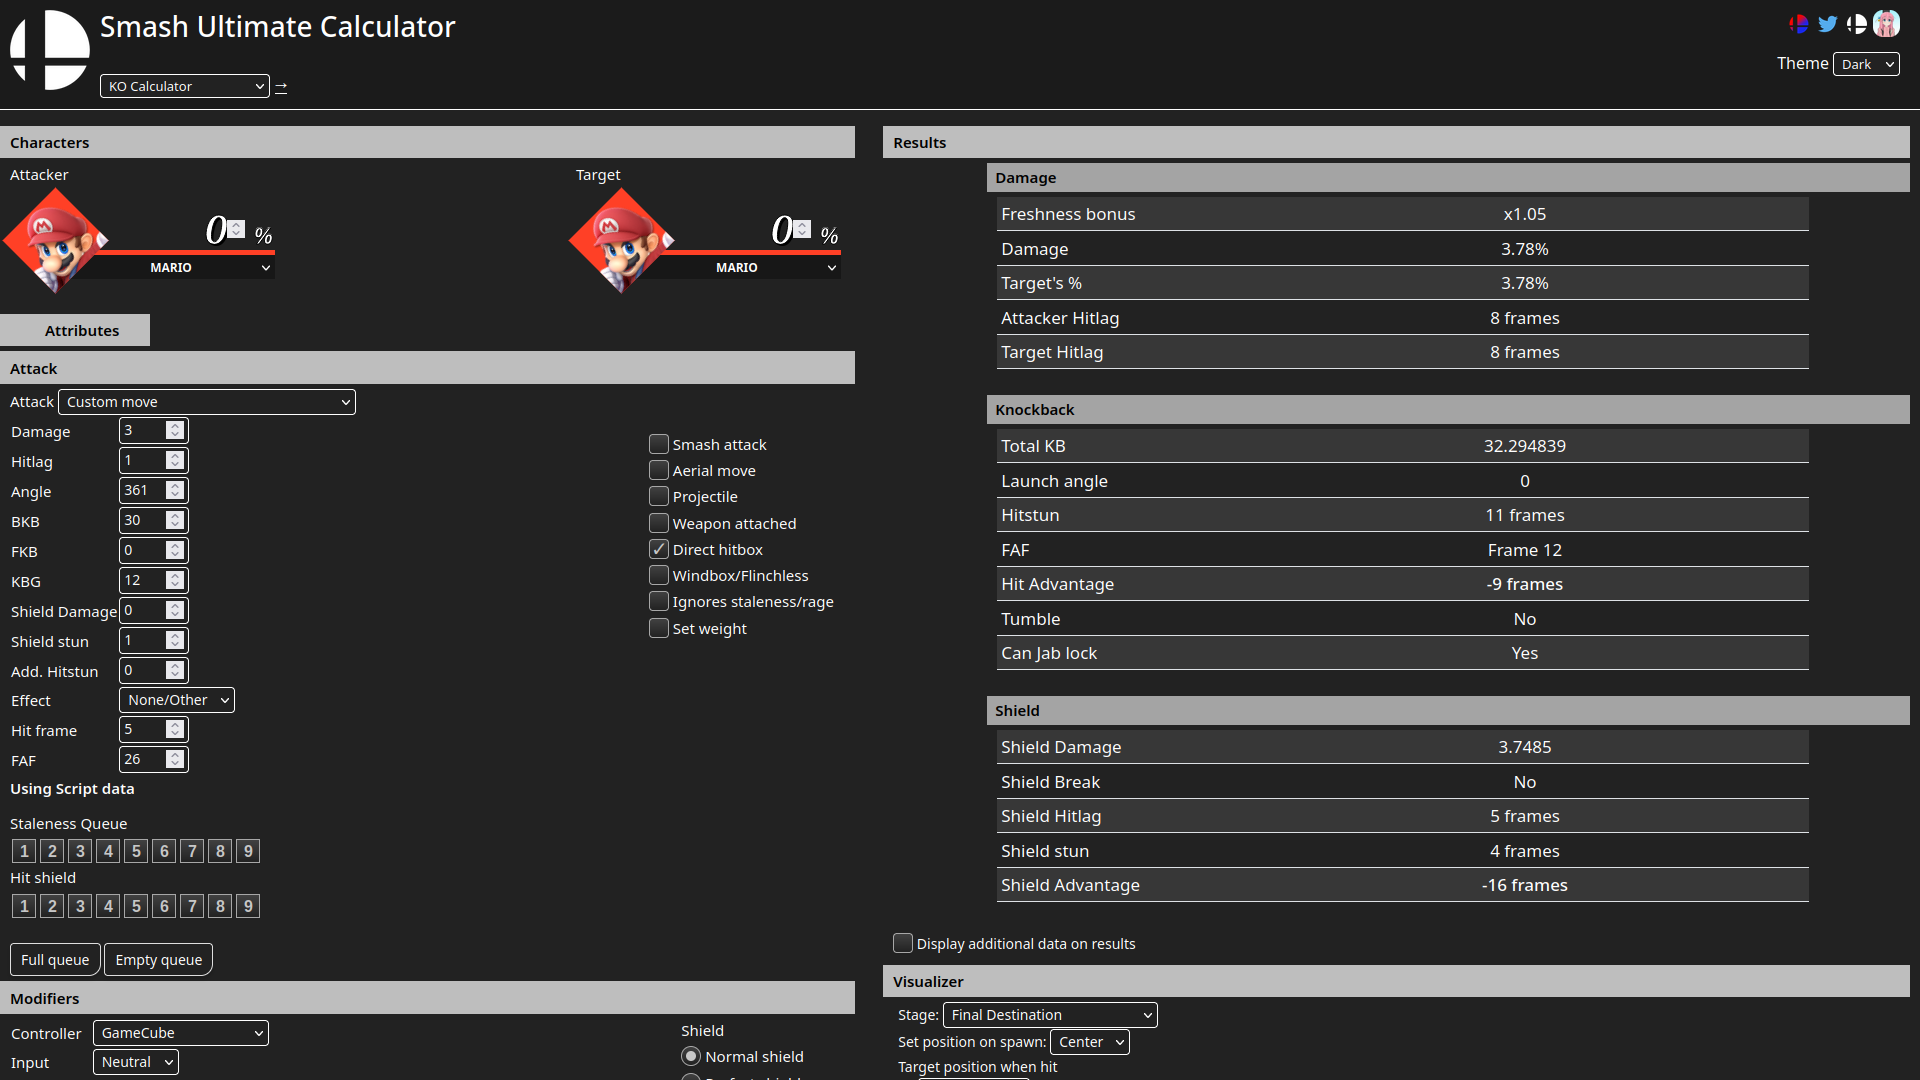
\includegraphics[width=0.75\textwidth]{figures/SUC1.png}
    \caption{Menú principal de \textit{Smash Ultimate Calculator}}
    \label{fig: SUC main menu}
\end{figure}

\begin{figure}[ht!]
    \centering
    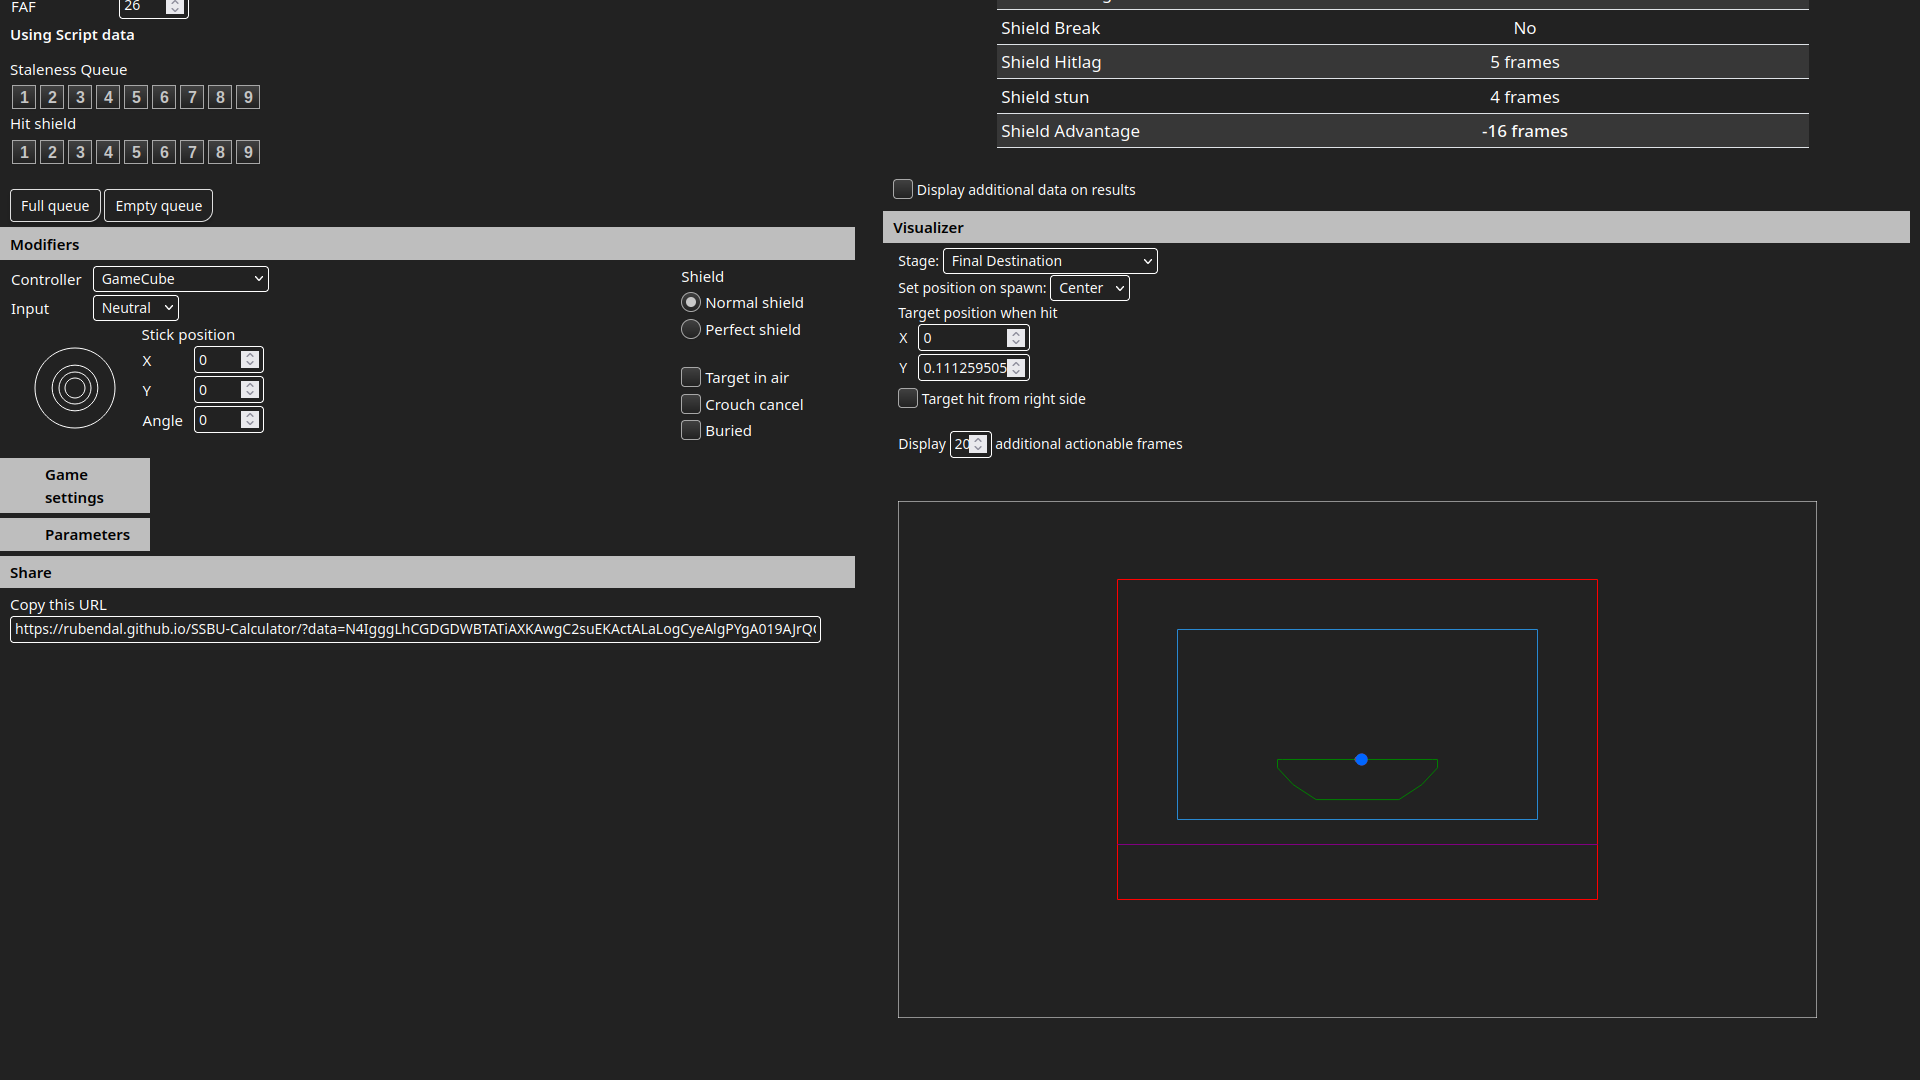
\includegraphics[width=0.75\textwidth]{figures/SUC2.png}
    \caption{Opciones adicionales de \textit{Smash Ultimate Calculator}}
    \label{fig: SUC additional options}
\end{figure}

\newpage

\textbf{Definición de Aspectos de la IGU}: 

% \begin{itemize}
%     \item Objetos
%     \item Acciones de la interfaz gráfica de usuario
%     \item Iconos
%     \item Vistas
%     \item Representaciones visuales de los objetos
%     \item Menú de los Objetos
%     \item Ventanas
% \end{itemize}

\textbf{Estructura de la interfaz gráfica de usuario}:

\begin{itemize}
    \item Los objetos actuales en la aplicación sería en su mayoría los botones, de los cuales los usuarios esperan que su funcionalidad este atada al botón correspondiente a tanto su lugar, como la acción que marca hacer.
    \item Las acciones que la interfaz gráfica permite para el usuario son:
    \begin{itemize}
        \item Presionar los objetos (botones)
        \item Desplegar la lista de opciones con estos
        \item Interactuar con ello tanto por entrada de teclado como un dispositivo apuntador
        \item Seleccionar sus opciones de la lista proveída en los botones
        \item Desplegar la pantalla para tanto leer instrucciones y los resultados de las comparaciones
    \end{itemize}
    \item Cada botón se representa como una caja rectangular con texto escrito encima del mismo. Esto se hace con el propósito de darle un contexto para qué se debe presionar dicha caja. Entre ellos, nombres, nombres de movidas y el botón de comparación para ver los resultados a base de las selecciones previas.
    \item Las vistas proveídas al usuario son 3:
    \begin{itemize}
        \item La primera y principal vista, selección de personajes
        \item La vista de instrucciones
        \item La vista de resultados en base a la selección de objetos
    \end{itemize}
    \item Cada objeto es representado con una imagen o representación propia por separado. En el caso de SkyboundDB, se utiliza una imagen del personaje junto al objeto de selección de personaje para que el usuario sepa quién esta escogiendo en tiempo dinámico. En cuestión al botón de comparación, este objeto se representa luego de que se haya presionado, pues es en base a que haya información para poder hacer las comparaciones y luego presentarlas de manera tabulada y con color al usuario. Cada uno de estos están envueltos en una caja rectangular para distinguirlos.
    \item Las secciones de selección y de comparación están divididas en dos menús rectangulares, uno superior y otro inferior. Mientras la opción de comparación no se ha hecho, este entonces es llenado con instrucciones de uso para el usuario, y luego es ocultado para presentar la información pertinente a la comparación.
    \item Todo se trabaja funcionalmente mediante una sola ventana, la cual es denominada por su titulo en HTML como \textit{SkyboundDB 2.0}.
\end{itemize}

\section{Prototipo}
\addcontentsline{toc}{section}{Prototipo}



\href{https://aramis-matos.github.io/skyboundDB2.0/}{SkyboundDB 2.0}

\begin{center}
    \begin{figure}[ht!]
        \centering
        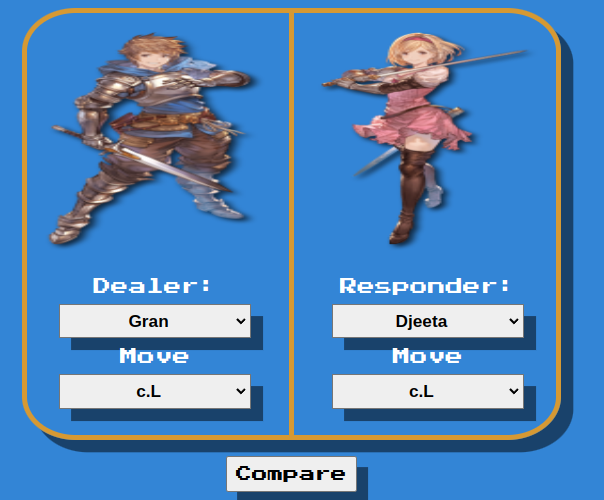
\includegraphics[height=0.4\textheight]{figures/Character_select_menu-object.png}
        \caption{Menú de objetos, iconos y representaciones visuales de los objetos del prototipo de selección de personajes}
        \label{fig: char sel prt}
    \end{figure}
\end{center}
  
    Aquí tenemos la representación visual de los objetos del prototipo de selección de personajes, donde podemos ver que presentamos a tanto el personaje encima del botón de selección de personaje (representado por un icono como un rectangulo), al igual que la selección de movida presentado de la misma manera. Por ello, se dedice presentar de lado a cada uno (como un espejo) las opciones del usuario, simulando la metáfora mencionada de cómo la selección de personajes se lleva a cabo en un juego de pelea tradicional, al igual que distinguir claramente entre quien \textbf{hace} la movida seleccionada y quien \textbf{responde} la movida con su  opción para contraatacar. Por último, vemos la opción de comparación presentado de manera consistente con el resto de los iconos para los objetos de selección (como una caja rectangular) fuera y debajo de la sección superior de menú de seleccíon de personaje y movida.

\begin{center}
    \begin{figure}
        \centering
        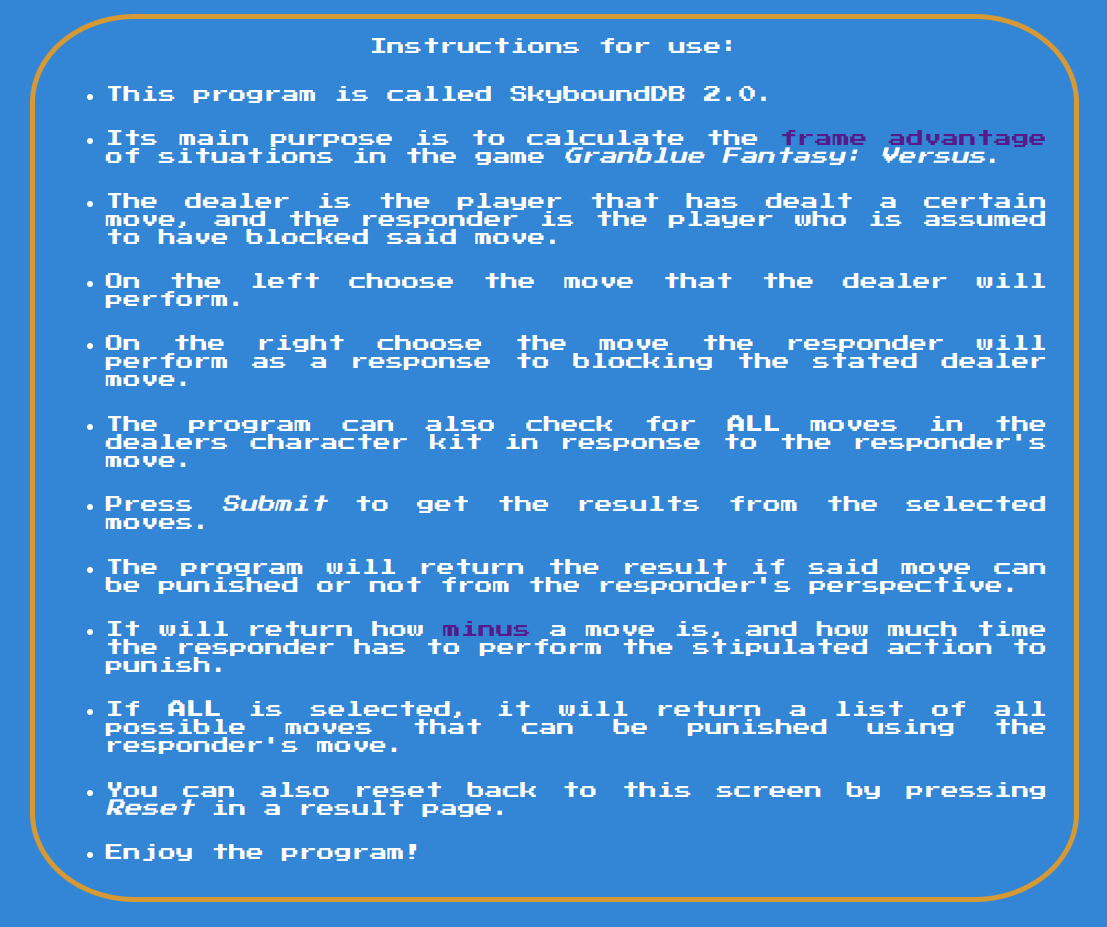
\includegraphics[height=0.4\textheight]{figures/Instructions_menu-object.png}
        \caption{Menú de instrucciones para el usuario}
        \label{fig: ins prt}
    \end{figure}
\end{center}

\newpage
    Se presenta las instrucciones del programa al usuario de la misma manera que se presenta cualquier menú en el programa, aislado en un rectangulo en su respectiva sección (en este caso, siendo la sección inferior del programa). Se muestran instrucciones de las opciones que el usuario tiene, definiciones y uso de la sección superior y el propósito de la aplicación. También se le provee terminología que es necesario entender para poder interpretar la información que el programa devuelve correctamente. Este menú es temporero, pues una vez se tome la primera acción, \textbf{no vuelve a aparecer} en excepción a que el usuario refresque la pagina nuevamente, puesto que este menú es reemplazado por el menú de resultados.

\begin{center}
    \begin{figure}
        \centering
        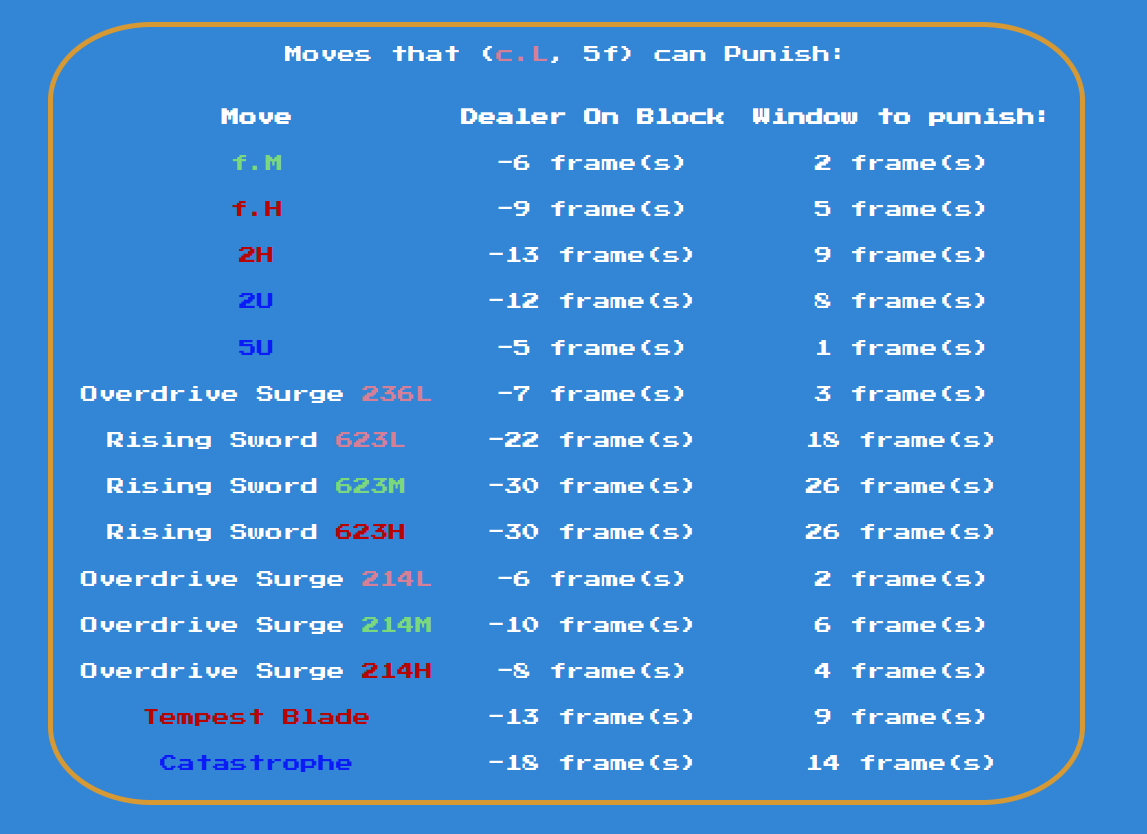
\includegraphics[height=0.4\textheight]{figures/Results_menu-object.png}
        \caption{Menú de resultados}
        \label{fig: rslt prt}
    \end{figure}  
\end{center}

\newpage
    Se le demuestra al usuario el menú de resultado en la parte inferior del programa, reemplazando el espacio previo de las instrucciones para el programa. Se implementa nuevamente el uso de un rectangulo aislando la información, pero esta vez se provee maneras de mantener la información facil de leer y compactada. Se producen los resultados en base a la selección de los objetos previos de personaje y de movida con colores de cada movida demostradas de manera similar que en el juego, como asi los resultados de las calculaciones. En este  prototipo, se enseña un ejemplo hipotético de Gran Vs Djeeta, todas las movidas de Gran contaatacadas con el c.L de Djeeta. Por último, se le presenta el usuario la opción de \textit{Reset} en vez de \textit{Compare} como el icono que se reemplaza en la sección superior del programa, pues se tiene que refrescar el menú inferior nuevamente para tomar nueva información y ejecutar otra comparación.

